\documentclass[12pt, a4paper]{article}
\usepackage[utf8]{inputenc}
\usepackage[margin=1in]{geometry}
\usepackage{amsmath}
\usepackage{graphicx}
\usepackage{booktabs}
\usepackage{hyperref}
\usepackage{listings}
\usepackage{xcolor}
\usepackage{tikz}
\usetikzlibrary{shapes.geometric, arrows, positioning}

% University Theme Colors
\definecolor{primaryColor}{RGB}{0,0,0}
\definecolor{secondaryColor}{RGB}{255,0,0}
\definecolor{backcolour}{rgb}{0.96,0.96,0.96}
\definecolor{codegreen}{rgb}{0,0.5,0}
\definecolor{codegray}{rgb}{0.5,0.5,0.5}
\definecolor{codepurple}{rgb}{0.58,0,0.82}

% Setup links
\hypersetup{
    colorlinks=true,
    linkcolor=secondaryColor,
    filecolor=primaryColor,      
    urlcolor=secondaryColor,
    pdftitle={Edge AI Lab Manual},
}

% Code Listing Style
\lstdefinestyle{mystyle}{
    backgroundcolor=\color{backcolour},   
    commentstyle=\color{codegreen},
    keywordstyle=\color{secondaryColor},
    numberstyle=\tiny\color{codegray},
    stringstyle=\color{codepurple},
    basicstyle=\ttfamily\footnotesize,
    breakatwhitespace=false,         
    breaklines=true,                 
    captionpos=b,                    
    keepspaces=true,                 
    numbers=left,                    
    numbersep=5pt,                  
    showspaces=false,                
    showstringspaces=false,
    showtabs=false,                  
    tabsize=2
}
\lstset{style=mystyle}

% TikZ Styles
\tikzstyle{process} = [rectangle, minimum width=3cm, minimum height=1cm, align=center, draw=primaryColor, fill=gray!10, text=primaryColor, thick, rounded corners]
\tikzstyle{arrow} = [thick,->,>=stealth, secondaryColor]

\title{\textbf{\Huge Edge AI \& TinyML Lab Manual} \\ \vspace{0.5cm} \Large CSE 521: Embedded Machine Learning}
\author{\textbf{Omar Tahon} \\ ID: 022025001}
\date{\today}

\begin{document}

\maketitle

\begin{abstract}
This lab manual introduces the concepts, models, and workflows associated with Edge Artificial Intelligence (Edge AI) and TinyML. We explore state-of-the-art architectures optimized for mobile and edge deployments, such as YOLOv11 and MobileNetV4, and delve into small language models (SLMs) like Phi-3. Furthermore, we investigate model compression via quantization and provide practical, self-contained experiments demonstrating how to quantize models and deploy them using tools such as the Texas Instruments \texttt{edgeai-tensorlab} ecosystem.
\end{abstract}

\tableofcontents
\newpage

\section{Introduction to Edge AI \& TinyML}
Edge AI involves running machine learning algorithms locally on hardware devices (the "edge" of the network) rather than relying on centralized cloud servers. This paradigm shift addresses several critical challenges in modern computing:
\begin{itemize}
    \item \textbf{Latency:} Processing data locally ensures real-time responses, crucial for autonomous driving and robotics.
    \item \textbf{Bandwidth:} Sending raw data (like high-res video) to the cloud is expensive; edge AI extracts insights locally.
    \item \textbf{Privacy \& Security:} Sensitive user data does not need to leave the device.
    \item \textbf{Power Efficiency:} TinyML specifically focuses on deploying models on ultra-low power microcontrollers (MCUs) consuming milliwatts of power.
\end{itemize}

\section{State-of-the-Art Edge Models}

\subsection{Vision Models: YOLOv11 and MobileNetV4}
Recent advancements have drastically reduced the size and computational requirements of vision models without significantly sacrificing accuracy.

\textbf{YOLOv11 (November 2024):} The latest iteration of the YOLO family introduces a transformer-based backbone with Partial Self-Attention (PSA) and NMS-free training. This results in a 25-40\% lower latency compared to its predecessors while achieving 60+ FPS processing on edge devices.

\textbf{MobileNetV4:} Developed by Google, MobileNetV4 introduces the Universal Inverted Bottleneck (UIB) block and Mobile MQA attention. It achieves 87\% ImageNet accuracy with merely 3.8ms latency on mobile edge TPUs, making it a universal efficient architecture for the mobile ecosystem.

\subsection{Small Language Models (SLMs)}
Large Language Models (LLMs) like GPT-4 are too massive for edge deployment. Instead, the industry is pivoting towards highly optimized SLMs:
\begin{itemize}
    \item \textbf{Microsoft Phi-3:} A 3.8B parameter model optimized for CPU and mobile inference, supporting up to 128K context windows.
    \item \textbf{TinyLlama:} A 1.1B parameter model with a highly compact architecture, designed specifically for low-resource environments.
\end{itemize}

\section{Model Compression and Quantization}
To fit these models onto constrained hardware, compression techniques are mandatory. Quantization maps high-precision floating-point numbers (FP32) to lower-precision representations (INT8, INT4).

\subsection{Quantization Techniques}
\begin{itemize}
    \item \textbf{Post-Training Quantization (PTQ):} The model is trained in FP32, and weights/activations are mapped to INT8 post-training. Simple but can degrade accuracy on complex tasks.
    \item \textbf{Quantization-Aware Training (QAT):} The model simulates low-precision behavior during training, learning to compensate for quantization noise, preserving accuracy.
    \item \textbf{Advanced Techniques (AWQ, GPTQ):} Activation-aware Weight Quantization (AWQ) protects salient (critical) weights from quantization, maintaining high accuracy even at 4-bit precision.
\end{itemize}

\section{Experiment 1: Model Quantization}
This experiment demonstrates how to simulate quantization on a randomly generated weight matrix using standard numerical libraries. It mirrors the fundamental operations happening inside inference engines.

\subsection{Code Implementation}
\begin{lstlisting}[language=Python, caption=Simulating INT8 Quantization in Python]
import numpy as np

def quantize_int8(weights):
    # Determine the dynamic range
    min_val = np.min(weights)
    max_val = np.max(weights)
    
    # Calculate scale and zero-point
    # INT8 range is [-128, 127]
    scale = (max_val - min_val) / 255.0
    zero_point = -128 - np.round(min_val / scale)
    
    # Quantize
    quantized_weights = np.round(weights / scale + zero_point)
    # Clip to valid INT8 range
    quantized_weights = np.clip(quantized_weights, -128, 127).astype(np.int8)
    
    return quantized_weights, scale, zero_point

def dequantize(quantized_weights, scale, zero_point):
    # Dequantize back to float32 for inference/computation
    return (quantized_weights.astype(np.float32) - zero_point) * scale

# 1. Generate dummy float32 weights
weights_fp32 = np.random.randn(10, 10).astype(np.float32) * 5

# 2. Quantize
weights_int8, scale, zp = quantize_int8(weights_fp32)

# 3. Analyze Compression Ratio
fp32_size = weights_fp32.nbytes
int8_size = weights_int8.nbytes
print(f"Compression Ratio: {fp32_size / int8_size}x") # Expected: 4.0x
\end{lstlisting}

\section{Experiment 2: End-to-End Edge Vision Deployment}
In this experiment, we explore the conceptual workflow of deploying a model using the \textbf{Texas Instruments \texttt{edgeai-tensorlab}} toolchain.

\subsection{The \texttt{edgeai-tensorlab} Workflow}
The TI ecosystem provides an end-to-end pipeline:
\begin{center}
    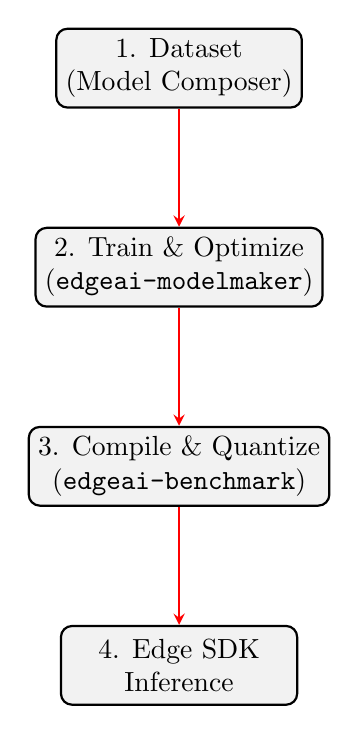
\begin{tikzpicture}[node distance=1.5cm]
        \node (data) [process] {1. Dataset \\ (Model Composer)};
        \node (train) [process, below=of data] {2. Train \& Optimize \\ (\texttt{edgeai-modelmaker})};
        \node (compile) [process, below=of train] {3. Compile \& Quantize \\ (\texttt{edgeai-benchmark})};
        \node (deploy) [process, below=of compile] {4. Edge SDK \\ Inference};

        \draw [arrow] (data) -- (train);
        \draw [arrow] (train) -- (compile);
        \draw [arrow] (compile) -- (deploy);
    \end{tikzpicture}
\end{center}

\subsection{Steps for Deployment}
\begin{enumerate}
    \item \textbf{Data Collection:} Use tools like EDGE-AI-STUDIO to capture and annotate images for a specific task (e.g., Object Detection).
    \item \textbf{Training via Bring Your Own Data (BYOD):} Use \texttt{edgeai-modelmaker} (a command-line tool wrapping around architectures like torchvision or mmdetection) to train a model. Model maker automatically handles architecture selection and hyperparameter tuning suitable for Edge processing.
    \item \textbf{Compilation and Benchmarking:} Pass the trained model to \texttt{edgeai-benchmark} or \texttt{edgeai-tidlrunner}. This step performs Post-Training Quantization (converting the model to fixed-point integers) and compiles the execution graph into machine code optimized for TI's neural processing units (NPUs).
    \item \textbf{Deployment:} The resulting compiled artifacts are deployed directly to the Edge AI SDK, executing inference pipelines via GStreamer plugins on the physical board.
\end{enumerate}

\section{Conclusion}
Edge AI is transforming how we deploy intelligence in the real world. By leveraging highly efficient model architectures (YOLOv11, MobileNetV4, Phi-3) and rigorous quantization strategies, modern engineering teams can extract real-time insights from sensor data without the latency, cost, and privacy concerns of cloud computing. Toolchains like \texttt{edgeai-tensorlab} abstract away the immense complexity of hardware compilation, allowing developers to focus on data and problem-solving.

\end{document}
